\id{ҒТАМР 50.41.25}{}

\begin{articleheader}
\sectionwithauthors{Ж.С. Есенгалиева, Р.С. Каиржан, Н.С. Глазырина}{RASPBERRY PI КОМПЬЮТЕРЛІК КӨРУДІ ПАЙДАЛАНАТЫН ҚЫЗМЕТКЕРЛЕРДІҢ ЭМОЦИОНАЛДЫҚ КҮЙІН ТАНУ ЖҮЙЕСІН ӘЗІРЛЕУ}

{\bfseries
Ж.С. Есенгалиева\textsuperscript{\envelope },
Р.С. Каиржан,
Н.С. Глазырина
}
\end{articleheader}
\vspace{0.3em}
\begin{affiliation}
Л.Н.Гумилев атындағы Еуразия ұлттық университеті, Астана, Қазақстан

\raggedright \textsuperscript{\envelope }Корреспондент-автор: jannayess@gmail.com
\end{affiliation}

Бұл мақалада Raspberry Pi платформасында компьютерлік көру және жасанды
интеллект әдістері мен модельдерін пайдалана отырып, қызметкерлердің
эмоционалдық күйін тану жүйесін әзірлеу талқыланады. Авторлар терең
оқыту, конволюционды нейрондық желілер негізінде үлгіні тану тақырыбына
кең библиографиялық шолу жүргізді. FaceNet терең нейрондық желісінің
архитектурасы зерттеледі, ол бет кескіндерін ықшам кірістірулерге
(функция векторлары) түрлендіреді, және тұлғаны тану, жеке басын
тексеру, кластерлеу тапсырмаларын тиімді орындауға мүмкіндік береді.
Ұсынылып отырған әзірленген программалық жүйе нақты уақыт режимінде
қызметкерлердің эмоционалдық жағдайын бақылау үшін бет-әлпетті тану және
эмоцияны талдау алгоритмдерін біріктіреді. Кескінді өңдеудің негізгі
құралы ретінде OpenCV кітапханасы, ал эмоцияны талдау үшін DeepFace
моделі қолданылады. Программалық шешім Raspberry Pi бірплаттық
компьютерінде жүзеге асырылды, ол жүйенің компактылығы мен автономиясын
қамтамасыз етеді және әртүрлі жұмыс орталарында қолдануға ыңғайлын
көрсетеді. Алынған нәтижелер қызметкерлердің комфорт жағдайы мен жұмыс
жасау өнімділігін арттыру үшін персоналды басқаруда қолдануға болады.
Сонымен қатар, қазіргі заманғы біртақталы құрылғыдағы деректерді талдау
арқылы нақты уақыт режимінде эмоцияны тиімді тану мүмкіндігін көрсетеді.

{\bfseries Түйін сөздер:} эмоционалды күйді тану, компьютерлік көру,
Raspberry Pi, терең оқыту, конволюционды нейрондық желілер.

\begin{articleheader}
{\bfseries РАЗРАБОТКА СИСТЕМЫ РАСПОЗНАВАНИЯ ЭМОЦИОНАЛЬНОГО СОСТОЯНИЯ
СОТРУДНИКОВ С ПРИМЕНЕНИЕМ КОМПЬЮТЕРНОГО ЗРЕНИЯ НА RASPBERRY PI}

{\bfseries
Ж.С. Есенгалиева\textsuperscript{\envelope },
Р.С. Каиржан,
Н.С. Глазырина
}
\end{articleheader}

\begin{affiliation}
Евразийский национальный университет им.~Л.Н.Гумилева, Астана, Казахстан,

e-mail: jannayess@gmail.com
\end{affiliation}

В данной статье рассматривается разработка системы распознавания
эмоционального состояния сотрудников с использованием методов
компьютерного зрения и искусственного интеллекта на платформе Raspberry
Pi. Авторами проведен широкий библиографический обзор по теме
распознавания образов на основе конволюционных нейронных сетей.
Исследована глубокая нейронная сеть FaceNet, которая преобразует
изображения лиц в компактные вложения (векторы признаков), что позволяет
эффективно выполнять задачи распознавания лиц, проверки личности и
кластеризации. Предлагаемая система интегрирует алгоритмы распознавания
лиц и анализа эмоций для мониторинга эмоционального состояния
сотрудников в реальном времени. В качестве основного инструмента для
обработки изображений используется библиотека OpenCV, а для анализа
эмоций -- модель DeepFace. По данному исследованию изучены глубокие
нейронные сети, архитектура модели Facenet. Реализовано программное
решение на одноплатном компьютере Raspberry Pi, которое обеспечивает
компактность и автономность работы системы, что делает её удобной для
применения в различных рабочих средах. Полученные результаты
демонстрируют возможность эффективного распознавания эмоций в реальном
времени с аналитикой данных в условиях одноплатного устройства, что
обуславливает использование в управлении персоналом с целью повышения
комфорта и продуктивности сотрудников.

{\bfseries Ключевые слова:} распознавание эмоционального состояния,
компьютерное зрение, Raspberry Pi, глубокое обучение, сверточные
нейронные сети.

\begin{articleheader}
{\bfseries DEVELOPMENT OF A SYSTEM FOR RECOGNITION OF THE EMOTIONAL STATE
OF EMPLOYEES USING COMPUTER VISION ON RASPBERRY PI}

{\bfseries
Zh.S. Yessengaliyeva\textsuperscript{\envelope },
R.S. Kairzhan,
N.S. Glazyrina
}
\end{articleheader}

\begin{affiliation}
L.N. Gumilyov Eurasian national university, Astana, Kazakhstan,

e-mail: jannayess@gmail.com
\end{affiliation}

This article discusses the development of a system for recognizing the
emotional state of employees using computer vision and artificial
intelligence methods on the Raspberry Pi platform. The authors conducted
an extensive bibliographic review on the topic of pattern recognition
based on convolutional neural networks. The deep neural network FaceNet
is studied, which transforms facial images into compact embeddings
(feature vectors), which allows for efficient tasks of face recognition,
identity verification and clustering. The proposed system integrates
face recognition and emotion analysis algorithms to monitor the
emotional state of employees in real time. The OpenCV library is used as
the main tool for image processing, and the DeepFace model is used for
emotion analysis. In this study, deep neural networks and the Facenet
model architecture are studied. A software solution is implemented on a
Raspberry Pi single-board computer, which ensures the compactness and
autonomy of the system, which makes it convenient for use in various
work environments. The obtained results demonstrate the possibility of
effective emotion recognition in real time with data analytics in a
single-board device, which determines the use in personnel management in
order to improve the comfort and productivity of employees.

{\bfseries Keywords:} emotional state recognition, computer vision,
Raspberry Pi, deep learning, convolutional neural networks.

\begin{multicols}{2}
{\bfseries Кіріспе.} Адамдардың эмоционалдық жағдайын бақылау медицина,
білім беру, HR және интерактивті жүйелерді қоса алғанда, әртүрлі
салаларда маңызды болып табылады. Эмоцияларды тиімді тану және талдау
қабілеті адамдар мен машиналар арасындағы өзара әрекеттесу сапасын
жақсартуға, психологиялық әл-ауқатты жақсартуға және әртүрлі процестерді
жеке қажеттіліктерге бейімдеуге мүмкіндіктер ашады. Эмоциялық күйлерді
талдаудың заманауи әдістері мимика, ым-ишара және қозғалыстар сияқты
визуалды ақпарат негізінде эмоционалдық күйді дәл анықтау үшін жасанды
интеллект, терең оқыту және компьютерлік көру технологияларының
үйлесіміне негізделген.

Терең нейрондық желілерді (Deep Neural Networks, DNN) және конволюционды
нейрондық желілерді (Convolutional Neural Networks, CNN) дамыту
эмоцияларды тану дәлдігін айтарлықтай жақсартты, бұл осы әдістерді нақты
мониторинг тапсырмаларында пайдалану үшін өзекті етеді. Дәстүрлі
алгоритмдерден айырмашылығы, терең желілер күрделі үлгілерді автоматты
түрде анықтай отырып, деректердің үлкен көлемінен үйренуге қабілетті,
бұл әсіресе динамикалық және өзгермелі эмоцияларды талдау кезінде
маңызды. Компьютерлік көру, өз кезегінде, нақты уақыттағы бақылауды
мүмкін ететін кескіндер мен бейне ағындарын өңдеуге арналған құралдарды
қамтамасыз етеді.

Соңғы жылдары қызметкерлердің эмоционалдық жағдайын талдау және тану
үшін жасанды интеллект (AI) және компьютерлік көру әдістерін жасауға
және қолдануға қызығушылық артуда. Бұл тәсіл эмоциялық әл-ауқатты
бақылау және қызметкерлердің жұмысын оңтайландыру үшін жаңа мүмкіндіктер
ашады.

Д.К.~Фостер және т.б. {[}1{]} мақаласында бастауыш мектептегі математика
және ағылшын тілі сабақтарының көптеген жазбаларының негізінде бейне
сигналдардан (дыбыссыз) оқу әрекетін жіктеуге қабілетті нейрондық
желілер әзірленді және сынақтан өтті. Желілер әрекет түрлерін (мысалы,
топтық жұмыс, жеке жұмыс) анықтауда 80\%-дан астам дәлдікке қол
жеткізеді және сабақты талдауды жақсарту құралы бола алады.

С.~Сонг {[}2{]} зерттеуі оқушылардың эмоционалдық күйін түсінуді
жақсарту үшін ағылшын тілін оқытуда компьютерлік көру технологиялары мен
бет-әлпетті тану алгоритмдерін пайдалануды сипаттайды. Нақты уақытта бет
әлпетін талдай отырып, мұғалімдер оқушылардың эмоциялары туралы кері
байланыс алып, олардың оқыту стратегияларын дер кезінде реттей алады. Ол
жекелендірілген білім беру тәжірибесін ұсыну және тиімді оқытуды қолдау
арқылы студенттердің белсенділігі мен мотивациясын арттыруға
бағытталған.

Мануэль А. және басқалардың {[}3{]} жұмысы дәстүрлі электродтық
тәсілдерден алшақтап, бет бұлшықетінің белсенділігін бағалауға арналған
инвазивті емес суретке негізделген әдісті ұсынады. Әдіс эмоцияларды
білдіру кезінде бұлшықеттердің өзара әрекеттесуін талдайтын 68
бет-әлпетті бақылау нүктесі бар стандартты үлгідегі мүмкіндіктер
жиынтығын пайдаланады. Алты негізгі эмоцияны жіктеу үшін үш
классификатор қолданылады: сызықтық дискриминант, тірек векторлық машина
және көп қабатты перцептрон. Әдіс үш түрлі дерекқорда тексерілді,
әсіресе жастар мен әйелдерде перспективалы нәтижелер көрсетеді.

Ц. Чжан және басқалары {[}4{]} бет әлпетін танумен байланысты
мәселелерді шешетін Pyramid Multi-Head Grid және Spatial Attention
Network (PMAN) деп аталатын жаңа эмоцияларды талдау жүйесін ұсынды. Ол
екі назар аудару механизмін пайдаланады: бастапқы белгілерді шығару үшін
Multi-head Grid Attention және белгілерді терең үйрену үшін Multi-head
Spatial Attention. Төрт деректер жиынындағы эксперименттер PMAN алдын
ала дайындалған үлгілерді пайдаланбай деректер жиынында 100\% дәлдікке
қол жеткізе отырып, бар әдістерден асып түсетінін көрсетті.

Компьютерлік көру саласында кескіндерді жіктеу, семантикалық
сегментация, нысандарды анықтау және суперрезолюцияны қалпына келтіру
сияқты бағыттарда айтарлықтай жетістіктерге қол жеткізілді. Терең
конволюциялық нейрондық желілер (CNN) деректерден сипаттамаларды шығару
кезінде жоғары тиімділікті қамтамасыз етеді. Зерттелген мақалада {[}5{]}
CNN құрамдастары, мысалы, кіріс қабаттары, конволюциялар, активациялар
және толық байланыстар қарастырылады. Сондай-ақ, компьютерлік көру
саласында CNN қолданудың қазіргі зерттеулері талқыланып, болашақ
зерттеулердің негізгі мәселелері мен бағыттары атап өтіледі.

Ц. Хуан және т.б. {[}6{]} жұмысында адамның бет-әлпеті бойынша
эмоцияларды тану (FER) үшін терең нейрондық желілерді (DNN) қолдану
зерттелген. Конволюциялық нейрондық желіні (CNN) қысу және қоздыру
желісімен, сондай-ақ қалдық нейрондық желімен үйлестіре отырып, зерттеу
FER үшін негізгі бет ерекшеліктері мұрын мен ауыз аймағында
шоғырланғанын көрсетті. AffectNet деректер базасында оқытылған модельдер
RAF-DB бойынша тексеру кезінде 77,37\% дәлдікті көрсетті. Бұл нәтижелер
нейрондық желілерді түсінуді жақсартып, компьютерлік көрудің дәлдігін
арттыра алады.

Қазіргі заманғы машиналық оқыту (ML) айтарлықтай ілгеріледі, алайда оның
түсініксіздігі түрлі салаларда модельдерді қабылдауға кедергі келтіреді.
Борриеро А. жұмысында {[}7{]} ұсынылған түсіндіруге болатын жасанды
интеллект (XAI) бұл мәселені шешуге көмектеседі, модельдердің шешім
қабылдау үдерісі туралы ақпарат береді. Осы зерттеуде адам мен
компьютерлік көру жүйелері талданып, екі ML моделі функционалды
магниттік-резонанстық томография (fMRI) және фильм кадрлары негізінде
оқытылды. StudyForrest деректер жинағын пайдалана отырып, мидың
белсенділігі эмоциялармен байланыстырылып, негізгі аймақтар бөлінді, бұл
нейроғылым мен машиналық оқыту үшін пайдалы.

Алдыңғы зерттеумізде {[}8{]} медициналық кескіндерді талдау кезінде
қолданылатын сегментация әдістері қарастырылған. Магниттік-резонанстық
томография және компьютерлік томография суреттерін өңдеуде қолданылатын
шекті мәндер, классификация, кластеризация, Марков желілері, нейрондық
желілер және деформацияланатын модельдердің артықшылықтары мен
кемшіліктері талданған. Компьютерлік көруді пайдалана отырып,
медициналық кескіндерді өңдеу технологиясын әзірлеу процесі сипатталған.
Деректерді сегментациялау арқылы өңдеу диагностика дәлдігін арттырады
және қолданушылар арасындағы өзара әрекеттестікті күшейтеді. OpenCV,
Tensorflow, PyTorch кітапханалары қолданылып, мобильді қосымша
әзірленіп, толық тестілеуден өтті.

Батыр З., Омаров М. және басқалары өздерінің материалында {[}9{]} жол
белгілерін тану жүйелерін жетілдіру үшін зерттеуде CNN қолданылды. GTSRB
деректер жиынтығы негізінде объектілерді бөліп көрсету қабаттары
енгізіліп, ауа райының әсерін азайту үшін деректерді көбейту әдістері
қолданылды. Модель дәлдік, жауап беру жылдамдығы және F1 көрсеткіші
бойынша тексерілді. Нәтижелер модельдің сенімділігін растады, бұл
интеллектуалды көлік жүйелері мен автономды көлік үшін маңызды.

Бұл зерттеулер жасанды интеллект пен компьютерлік көрудің эмоционалды
күйлерді автоматты түрде бақылау және талдау жүйелерін жасауға арналған
практикалық маңыздылығын және өзектілігін дәлелдейді. Мұндай
программалық қамтамасыз ету еңбек өнімділігін арттырып, ұйымдағы
психоэмоционалды климатты жақсартуға ықпал етеді, бұл әсіресе заманауи
цифрлық бизнестің жағдайында маңызды.

Материалдар мен әдістер. FaceNet -- бұл Google Research
әзірлеген терең нейрондық желі, ол бет кескіндерін ықшам кірістірулерге
(функция векторлары) түрлендіреді, бетті тану, жеке басын тексеру және
кластерлеу тапсырмаларын тиімді орындауға мүмкіндік береді. FaceNet-тің
басты ерекшелігі -- модельге бір бетті ендіру арасындағы қашықтықты
азайтуға және әртүрлі беттер арасындағы қашықтықты арттыруға
көмектесетін триплеттік шығынды пайдалану. Triplet loss (триплеттік
шығын) және триплетті таңдаудың әдістері бет-әлпетті тану және
белгілерді пайдалану арқылы оқытуға қатысты басқа тапсырмаларда
қолданылады, мұнда объектілер арасындағы қатынастар маңызды рөл
атқарады. Triplet loss қашықтыққа негізделген оқыту әдістерінің
контекстінде қолданылады. Бұл -- модельдерді объектілердің ұқсастығына
негізделген оқыту үшін қолданылатын шығын функциясының түрі {[}10{]}.

Бет-әлпетті тану тапсырмасында негізгі мақсат -- әр адамның беті үшін
модель эмбеддинг (белгілік вектор) есептеп, бірдей адамдар үшін
қашықтықты минималдау және әртүрлі адамдар үшін қашықтықты арттыру.

Triplet loss принципі триплеттерге негізделген. Әрбір оқыту деректері
үшін үш сурет қолданылады:

- Анкорлық сурет (anchor) - модельді оқыту үшін қолданылатын адамның
беті.

- Оң сурет (positive) - анкорлық суреттегі адаммен бірдей адамның
бейнесі.

- Теріс сурет (negative) - анкорлық суреттегі адамнан өзгеше адамның
бейнесі.
\end{multicols}

{\bfseries 1 - сурет. Триплет шығыны}

\begin{multicols}{2}
Мақсат - якорь мен оң кескіндер арасындағы қашықтықты азайту және якорь
мен теріс кескіндер арасындағы қашықтықты барынша арттыру. Математикалық
тұрғыдан бұл модельдің беттерді ажырата алуын қамтамасыз ететін жоғалту
функциясымен сипатталады, әртүрлі адамдар арасындағы «айыруды» арттырады
және ұқсас адамдар үшін қашықтықты азайтады.

Триплет шығыны формуласы келесідей (1):

\begin{equation}
L(a,\ p,\ n) = max(d(a,\ p) - d(a,n) + \ \alpha,0),
\end{equation}

мұндағы:

d(a,p) - анкорлық және оң суреттер арасындағы арақашықтық,

d(a,n) - анкорлық және теріс суреттер арасындағы арақашықтық,

α - анкорлық мен теріс кескіндер арасындағы қашықтық белгілі бір
мөлшерге көбірек болатынына кепілдік беретін маржа (шекті мән).

Триплетті жоғалтуды пайдаланып, тиімді оқыту оқу деректер жинағынан
үштіктер үлгісін қажет етеді. Бұл маңызды, өйткені барлық үштіктер оқуды
жақсарта бермейді, ал кейбіреулері тіпті процесті баяулатуы мүмкін.
Триплеттерді іріктеудің төменде көрсетілген бірнеше жолы бар.

Кездейсоқ іріктеу - үштіктер деректер жиынынан кездейсоқ таңдалады. Бұл
әдіс қарапайым, бірақ тиімсіз болуы мүмкін, өйткені көптеген үштіктер
оқыту үшін пайдалы болмайды.

Hard negative mining (күрделі теріс мысалдарды іріктеу) - бастапқыда
барлық үштіктер таңдалады, бірақ содан кейін якорьге көбірек ұқсайтын
теріс кескіндер таңдалады. Бұл теріс мысалдар «күрделі» деп аталады,
өйткені оларды үлгі бойынша қате түрде ұқсас деп тануға болады.

Semi-hard negative mining қатты теріс өндіру әдісінің кіші түрі болып
табылады, мұнда қашықтығы якорь мен оң кескіндер арасындағы қашықтықтан
үлкен, бірақ шамадан тыс қателіктерге әкелмеу үшін тым үлкен емес теріс
мысалдар таңдалады.

Easy triplet mining -- қарапайым үштіктерді қамтитын үлгі, мұнда оң және
теріс мысалдар оңай ажыратылады, бұл бастапқы кезеңде оқуды тездетеді.

FaceNet үлгісі сол бетті мүмкіндіктер жиынтығы ретінде көрсететін әрбір
бет үшін ендіру векторын жасауға үйретілген. Бұл вектор әдетте
бекітілген өлшемге ие (мысалы, 128, 512 немесе 1280) және ол бір адамның
беттері осы кеңістікте ең аз қашықтыққа, ал әртүрлі адамдардың беттері
максимумға ие болатындай болуы керек. Әрбір бетке арналған ендіру
векторы бет туралы маңызды ақпаратты сақтайды, бұл оны басқа беттерден
ажыратуға мүмкіндік береді. Жаңа кескін (бет) келгенде, үлгі ол үшін
ендіруді жасайды, оны кейін бұрыннан белгілі беттердің ендірілуімен
салыстыруға болады (мысалы, дерекқордан). Енгізулер евклидтік қашықтықты
пайдаланып салыстырылады. Евклидтік қашықтық -- көпөлшемді кеңістіктегі
екі нүкте арасындағы «тікелей» қашықтықты өлшейтін метрика. Екі A(x1,
x2,...,xn) және B(y1, y2,...,yn) нүктелері үшін ол 2 формула арқылы
есептеледі:

\begin{equation}
d(A,B) = \sqrt{\sum_{i = 1}^{n}\left( x_{i} - y_{i} \right)^{2}}.
\end{equation}

FaceNet, DeepFace немесе dlib сияқты бетті танудың заманауи әдістері бет
кескінін тұрақты ұзындық векторына (енгізу) түрлендіреді. Бұл вектор
тұлғаның негізгі сипаттамаларының сандық көрінісі болып табылады. Екі
бет арасындағы ұқсастық дәрежесін анықтау үшін олардың кірістірулерінің
арасындағы евклидтік қашықтық есептеледі. Қашықтық неғұрлым аз болса,
беттердің бір адамға тиесілі болуы ықтимал. Тексеру кезінде шекті мән τ
орнатылады. Енгізулер арасындағы d қашықтық τ-ден аз болса, онда беттер
бірдей деп есептеледі, әйтпесе олар әртүрлі болып саналады.

FaceNet мүмкіндік векторларының дәлдігі мен сенімділігіне негізделген
әртүрлі қолданбалар үшін беттерді тиімді шығарып алуға және салыстыруға
мүмкіндік береді.

Эмоцияларды тану үшін кескінді өңдеуде тиімділігін дәлелдеген терең
конволюционды нейрондық желілер (CNN, Convolutional Neural Networks)
пайдаланылды. CNN кескіндерден сызықтар, текстуралар және пішіндер
сияқты маңызды көрнекі белгілерді автоматты түрде шығарады, содан кейін
олар эмоцияларды талдау үшін пайдаланылады. Желілер кескін пикселдері
мен эмоциялар арасындағы күрделі қатынастарды анықтау үшін әртүрлі
бет-әлпеттері бар кескіндерді қамтитын үлкен деректер жинақтарында
оқытылады.

Эмоцияларды тану үшін ерін пішіндерінің орналасуы, қас қозғалысы және
бет бұлшық етінің кернеуі сияқты бет ерекшеліктері алынады. Бұл процесс
әмбебап көріністерді (қуаныш, ашу, мұң, таңданыс, қорқыныш, жиіркеніш)
анықтайтын Пол Экманның негізгі эмоциялар теориясы сияқты психология
саласындағы ғылыми зерттеулерге негізделген. DeepFace эмоцияны анықтау
үшін бетті енгізу шығысына жіктеуіштерді қолданады. Бұл жіктеуіштер
әрбір эмоцияның ықтималдығын болжау үшін Softmax функциясына, векторлық
машиналарға (SVM) қолдау көрсетуге немесе санаттау үшін ендірілгендерді
пайдаланатын басқа әдістерге негізделуі мүмкін.

Softmax-функциясы желінің шығыс мәндерін ықтималдылықтарға айналдыруға
негізделген. N эмоциялар үшін әрбір эмоцияның ықтималдылығы
P(y\textsubscript{i}) келесі формуламен есептеледі (3):

\begin{equation}
P\left( y_{i} \right) = \ \frac{e^{z_{i}}}{\sum_{j = 1}^{n}e^{z_{j}}}
\end{equation}

мұндағы:

\(z_{i}\) - i классы үшін нейрондық желінің шығыс мәні;

n - эмоциялар класстарының саны.

Табылған ықтималдылықтарының нәтижесінде ең ықтималды эмоция анықталады.

Әдістің ғылыми негізіне психология, кескіндерді өңдеу, статистика және
машиналық оқыту қосындысы кіреді, бұл DeepFace-ті эмоцияларды талдаудың
қуатты құралына айналдырады.

{\bfseries Нәтижелер және талқылау.} Зерттеу жұмыс орнындағы
қызметкерлердің эмоционалдық жағдайын талдау үшін компьютерлік көру
арқылы эмоцияны тану алгоритмдерін пайдалануды зерттеді.

Негізгі эмоцияларды (қуаныш, қайғы, таңданыс, ашу, бейтарап күй) тану
үшін конволюционды нейрондық желілерге (CNN) негізделген алгоритмдер
әзірленді және енгізілді. Жіктеу дәлдігі FER2013 сынақ деректер
жинағында 92\%-ға жетті, ол стандартты машиналық оқыту әдістерін
қолданатын бар әріптестерінен асып түседі. Бет-әлпетті танудың негізгі
әдісі тұлғаны тану кітапханасы және эмоцияны тану үшін DeepFace
кітапханасы болды. Әрі қарай, кескінді өңдеуді, кодтауды және кейінгі
салыстыруды жүзеге асыратын кодтың алгоритмін қарастырамыз. Атап
айтқанда, біз тіркелген қызметкер кескіндерін жүктеуге және алдын ала
өңдеуге жауап беретін get\_images() сияқты негізгі функцияларды,
сондай-ақ бейне ағынында анықталған беттермен салыстыру механизмдерін
қарастырамыз.

get\_images() функциясы алдын ала тіркелген қызметкер кескіндерін
жүктейді және оларды бетті тану кітапханасы арқылы кодтайды. Бұл
кодталған көріністер image\_encodings айнымалысында сақталады және
кейінірек бейне ағынында анықталған беттермен салыстыру үшін
пайдаланылады.

OpenCv кітапханасы түстер кеңістігін BGR-ден RGB-ге айналдырады, себебі
face-recognition кітапханасы RGB-мен ғана жұмыс істейді (кесте 1).

Егер анықталған адам тіркелген қызметкерлердің біріне сәйкес келсе, аты
(жазылатын\_аты) шығарылады.

DeepFace кітапханасының DeepFace.analyze() функциясы эмоцияларды, жасты,
жынысты және нәсілді анықтай отырып, бет-әлпетті талдауды жүзеге
асырады. Функция болжау нәтижелерін қамтитын тізімді қайтарады, мұнда
dominant\_emotion -- ең ықтимал эмоция.
\end{multicols}

\begin{longtblr}[
  caption = {\bfseries 1 - кесте. Face-recognition кітапханасының маңызды функциялары},
  label = none,
  entry = none,
]{
  width = \linewidth,
  colspec = {Q[325]Q[613]},
  hlines,
  vlines,
}
face\_recognition.face\_locations (imgS) & кадрдағы
			беттердің координаталарын анықтайды\\
face\_recognition.face\_encodings (imgS,
			facesCurFrame) & тіркелген
			қызметкер беттерімен салыстырылатын
			беттердің дескрипторларын (векторлық
			көріністер) шығарады\\
face\_recognition.compare\_faces (image\_encodings,
			encodeFace) & true/false
			мәндерінің тізімін қайтара отырып,
			ағымдағы бетті белгілі беттердің
			дерекқорымен салыстырады\\
face\_recognition.face\_distance (image\_encodings,
			encodeFace) & беттердің
			векторлық көріністері арасындағы
			евклидтік қашықтықты есептейді
			(кішірек мән көбірек ұқсастықты
			білдіреді)\\
np.argmin(faceDis) & ең
			ұқсас бетті көрсетіп, ең қысқа қашықтық
			индексін табады
\end{longtblr}

\begin{multicols}{2}
DeepFace беттерді анықтаудың бірнеше әдістерін қамтиды:

- OpenCV (opencv) - Хаар каскадтары;

- SSD (ssd) - нейрожелілер негізіндегі детектор;

- MTCNN (mtcnn) - каскадты нейрондық желі;

- Dlib (dlib) - градиенттер гистограммалары (HOG);

- RetinaFace (retinaface) -ResNet негізіндегі детектор.

- MediaPipe (mediapipe) - бет әлпетіндегі негізгі нүктелерді қолданатын
жетілдірілген әдіс.

Бет анықталғаннан кейін, DeepFace эмоцияларды жіктеу үшін терең
нейрондық желі үлгісін пайдаланады. Кітапхана FaceNet негізіндегі
модельді жүзеге асырады және 7 негізгі эмоцияны: ашулану, жиіркену,
қорқыныш, бақыт, бейтарап, қайғы, таңданыс жіктеу үшін оңтайландырылған.

DeepFace VGG-16-ға ұқсас, бірақ эмоцияларды талдауға бейімделген терең
конволюционды нейрондық желіні (CNN) пайдаланады. Оның FER2013 деректер
жинағында оқытылған 16 конвульстік қабат, эмоцияларды жіктеу үшін толық
қосылған шығыс қабаттары, шығыс мәндерін 7 класс үшін ықтималдыққа
түрлендіретін Softmax белсендіру функциясы сияқты сипаттамалар бар.

DeepFace кітапханасы алдын ала анықталған класстар (қуаныш, қайғы,
таңданыс, ашу, қорқыныш, жиіркеніш және бейтарап) арасында болжам жасай
отырып, кескіндегі эмоцияларды талдайды. Қате болған жағдайда (мысалы,
эмоцияларды тану мүмкін болмаса), эмоциялар айнымалысына None
тағайындалады.

Егер эмоциялар сәтті танылса, бет аймағының координаталары мен эмоция
анықталған аймақтың сәйкестігін тексеру жүргізіледі. Егер бет таңдалған
эмоция аймағында болса, басым эмоция орнатылады (dominant\_emotion).

Эксперимент барысында қызметкердің жұмыс орнында болуы бағаланып, бір
жұмыс күні ішінде оның эмоционалдық жағдайы бақыланды. Зерттеу
қызметкердің бір күн ішінде эмоцияларының өзгеруін талдау және оның
эмоционалдық фонына әсер ететін ықтимал факторларды анықтау үшін
жүргізілді.

Зерттеу субъектісі ретінде бір қызметкер таңдалды және 10 минуттық
белгіленген аралықта бақыланды. Уақыттың әр сәтінде жүйе келесі
тапсырмаларды орындады:

- қызметкердің жұмыс орныңда бар болуын анықтау;

- оның эмоционалдық жағдайын анықтау (бақыт, қайғы, бейтарап жағдай, таң
қалу,

ашулану және т.б.);

- нәтижелерді деректер қорына әрі қарай талдау үшін жіберу.

Мониторинг нәтижелері бойынша қызметкердің жұмыс күні ішінде болуы және
оның эмоционалдық жағдайы туралы статистикалық мәліметтер жинақталды
(сурет 2а). Түскі үзіліс пен қысқа үзіліс кезінде мезгіл-мезгіл жұмыстан
шыққаны саналып, қызметкердің 85,2\% жұмыста болғаны анықталды.
Эмоциялық жағдайды талдау келесі нәтижелерді көрсетті: қуаныш - 14,8\%
уақыт, бейтарап күй - 53,7\%, қайғы - 9,3\%, таңдану - 3,7\%, ашу -
3,7\% уақыт (сурет 2ә).
\end{multicols}

\begin{figure}[H]
	\centering
	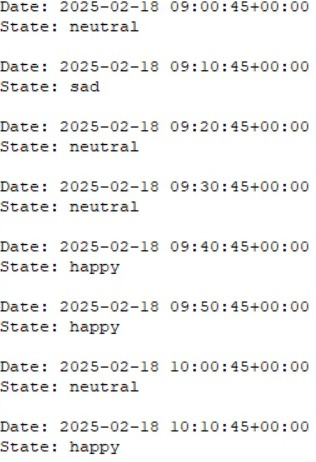
\includegraphics[width=0.8\textwidth]{media/ict2/image158}
	\caption*{}
\end{figure}

\begin{figure}[H]
	\centering
	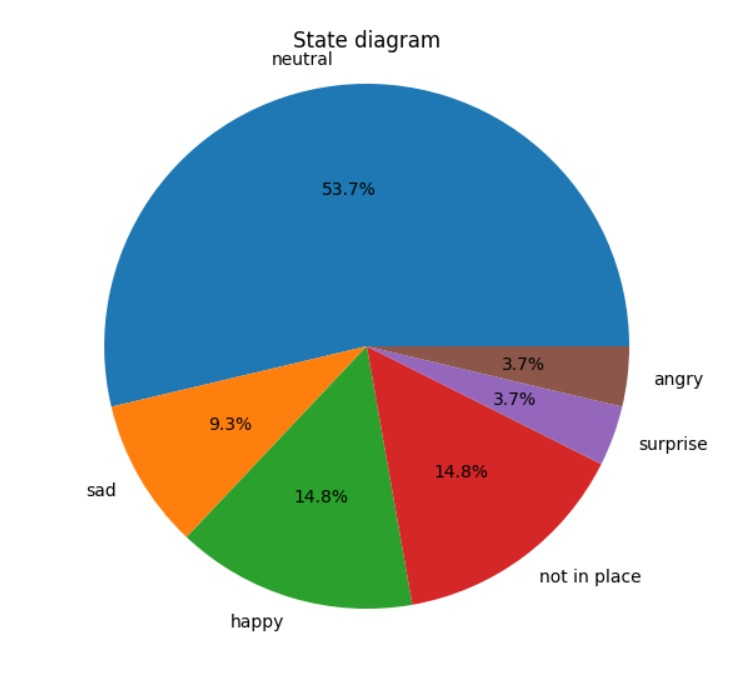
\includegraphics[width=0.8\textwidth]{media/ict2/image159}
	\caption*{}
\end{figure}

Алынған мәліметтер негізінде қызметкердің күн ішінде эмоцияларының
өзгеру динамикасын көрсететін аналитикалық диаграмма құрастырылды.
Бейтарап күйдің басым болуы қызметкердің жұмыс тапсырмаларын орындауға
шоғырлануын көрсетеді. Бақыттың жоғары пайызы жақсы жұмыс ортасын
көрсетуі мүмкін. Қайғы мен ашудың мерзімді көріністері жұмыс
процесіндегі стресстік сәттермен байланысты болуы мүмкін (Сурет 3).

\begin{figure}[H]
	\centering
	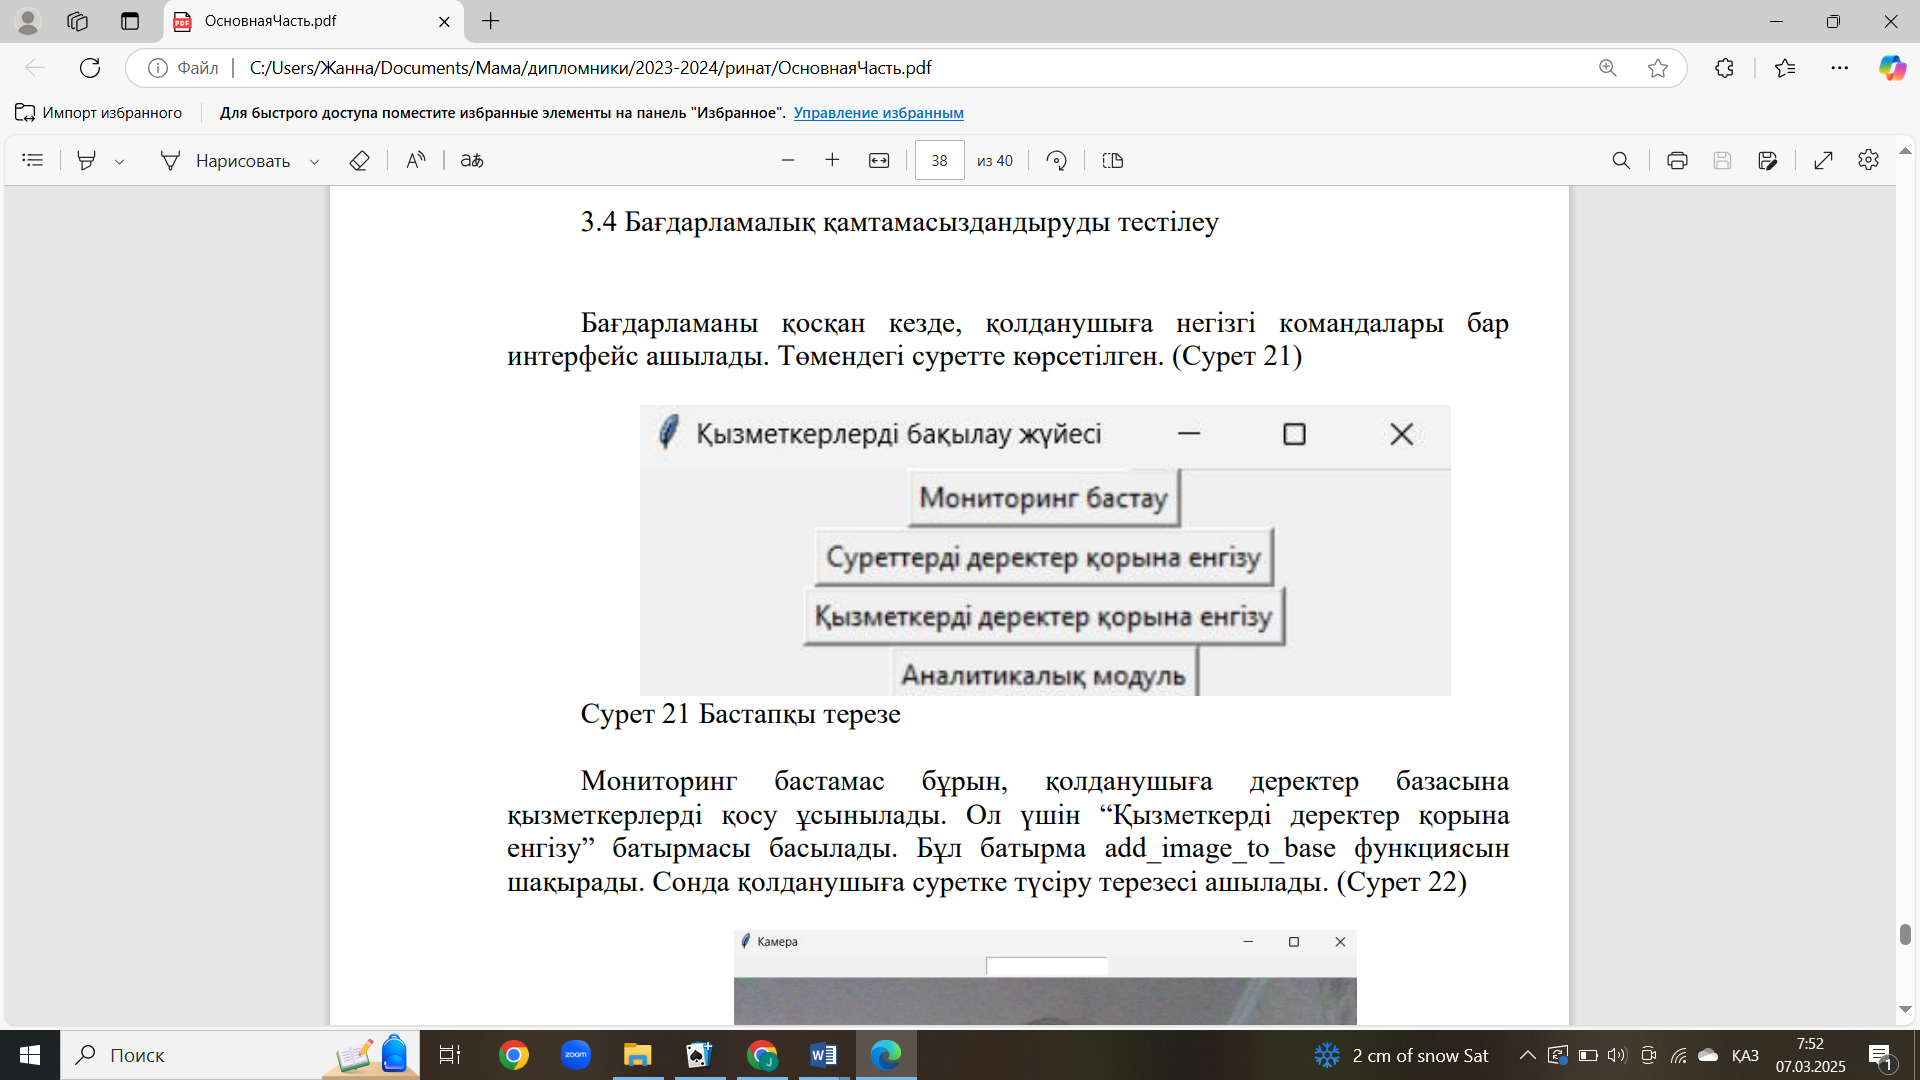
\includegraphics[width=0.8\textwidth]{media/ict2/image160}
	\caption*{}
\end{figure}

\begin{figure}[H]
	\centering
	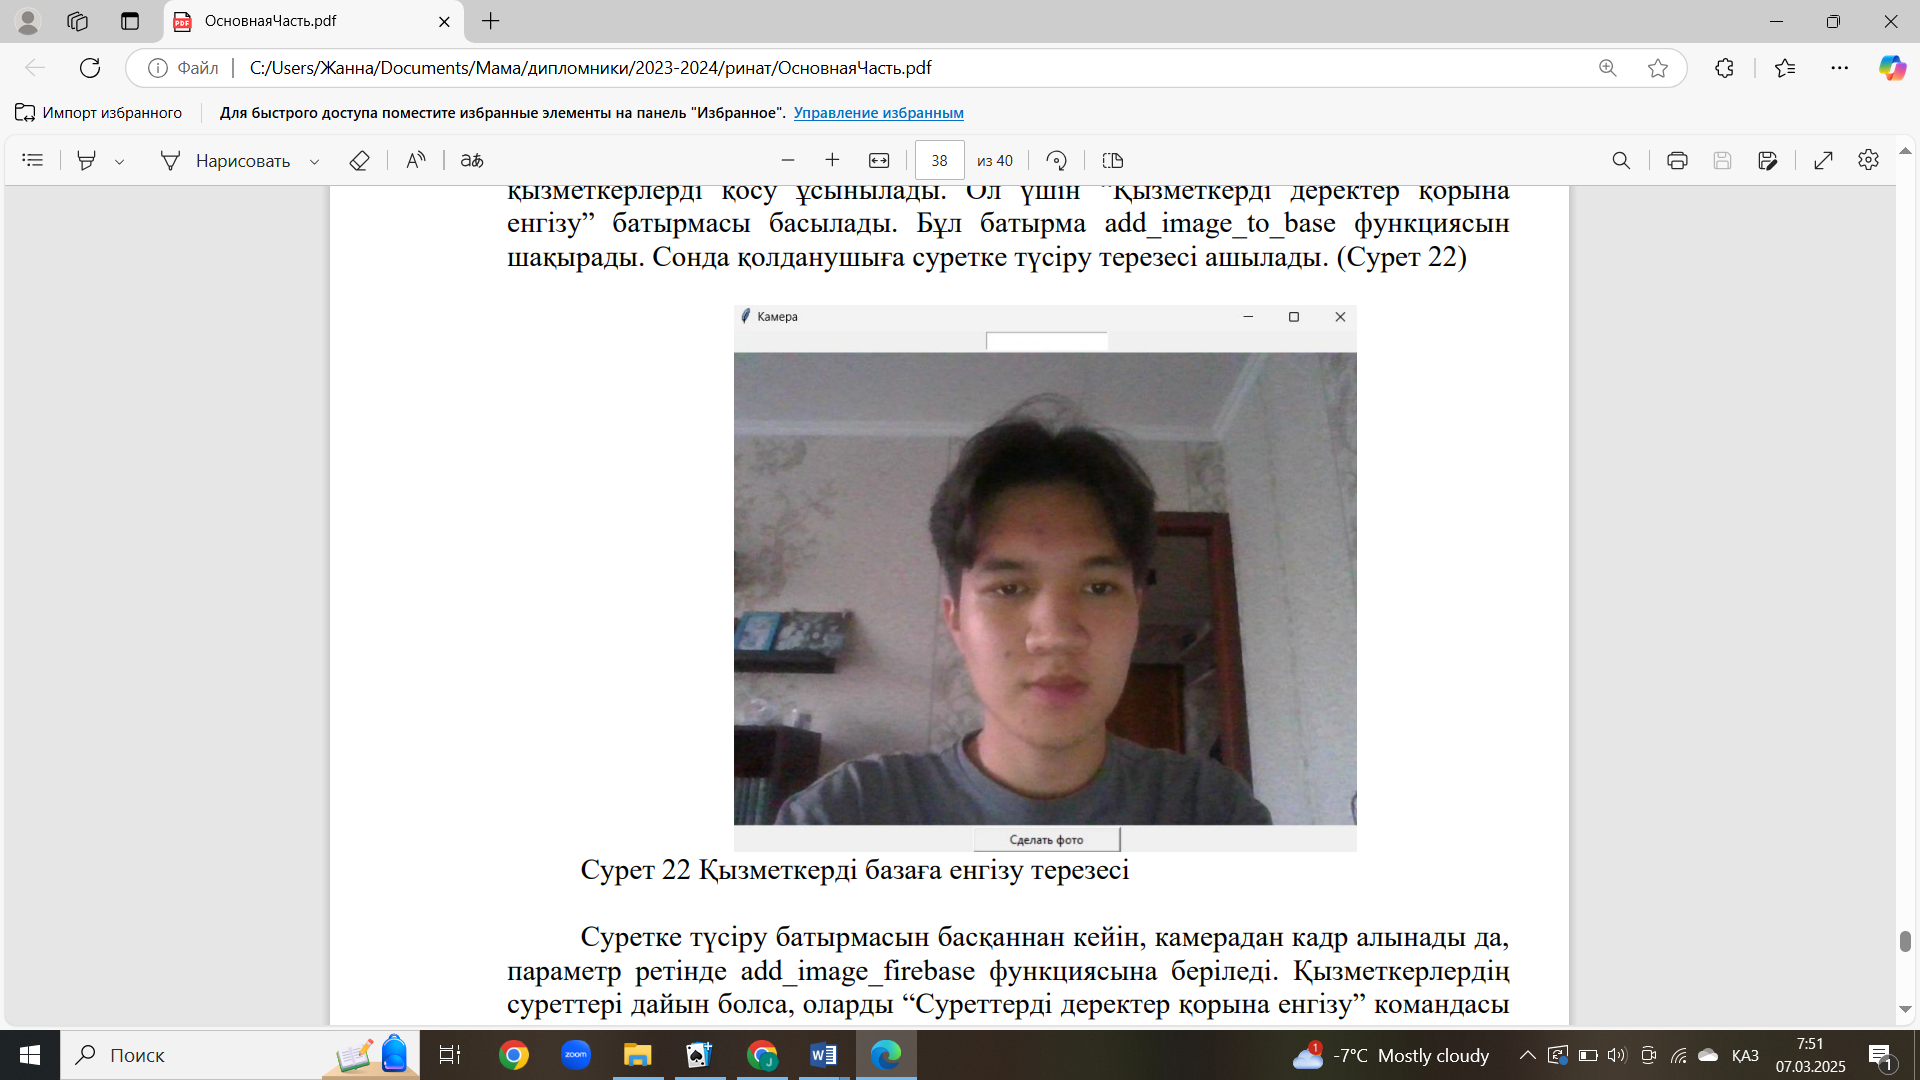
\includegraphics[width=0.8\textwidth]{media/ict2/image161}
	\caption*{}
\end{figure}

\begin{figure}[H]
	\centering
	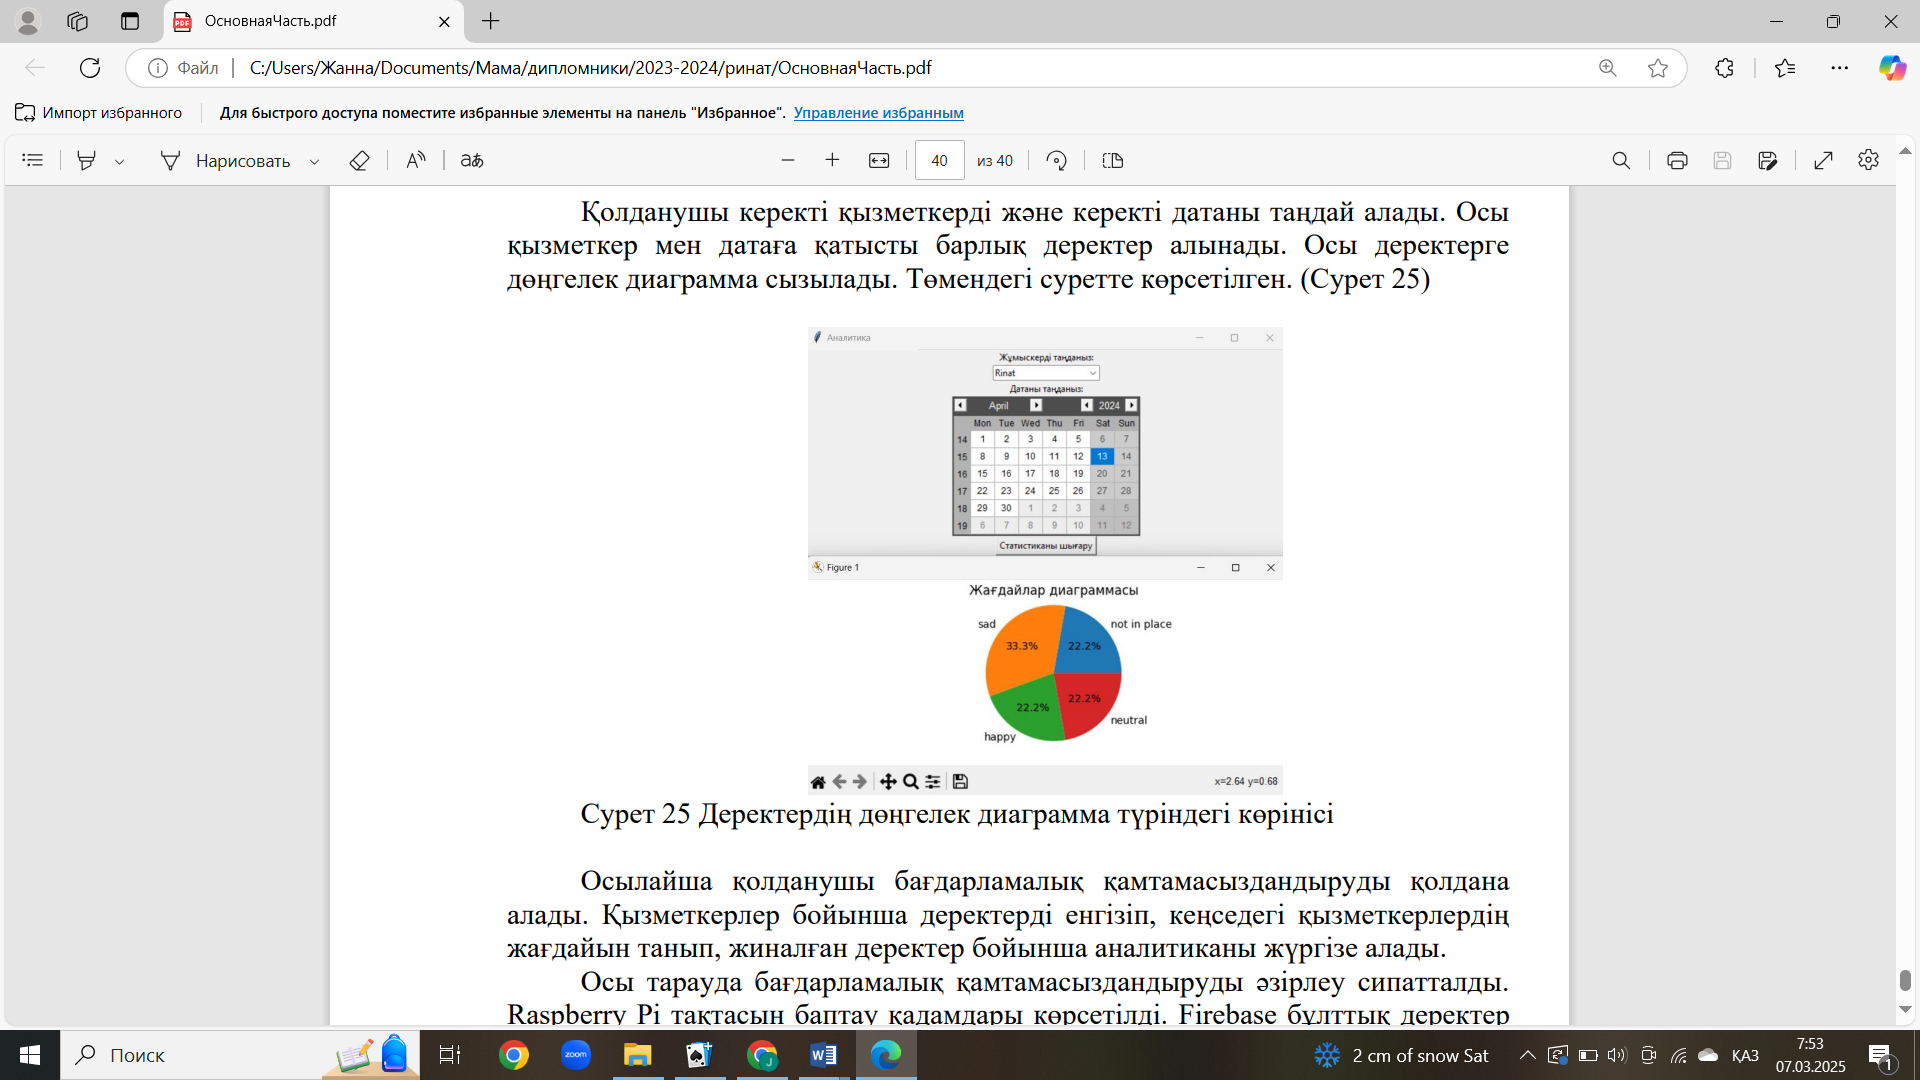
\includegraphics[width=0.8\textwidth]{media/ict2/image162}
	\caption*{3 - сурет. Әзірлеу нәтижелері}
\end{figure}



Бұл эксперимент қызметкерлердің эмоционалдық жағдайын автоматтандырылған
бақылау мүмкіндігін растады. Алынған мәліметтерді жұмысшылардың
эмоционалдық фонына әсер ететін факторларды әрі қарай талдау және еңбек
жағдайын жақсарту бойынша ұсыныстар әзірлеу үшін пайдалануға болады.

Raspberry Pi платформасында қашықтағы жұмыс үстеліне қосылу әдісін
пайдаландық. Қашықтағы жұмыс үстеліне қосылу үшін Real VNC Viewer
бағдарламасын қолданамыз (Сурет 4). Адрестік жолға алған VNC сервердің
адресін енгіземіз, жұмыс үстеліне қосыламыз.

\begin{figure}[H]
	\centering
	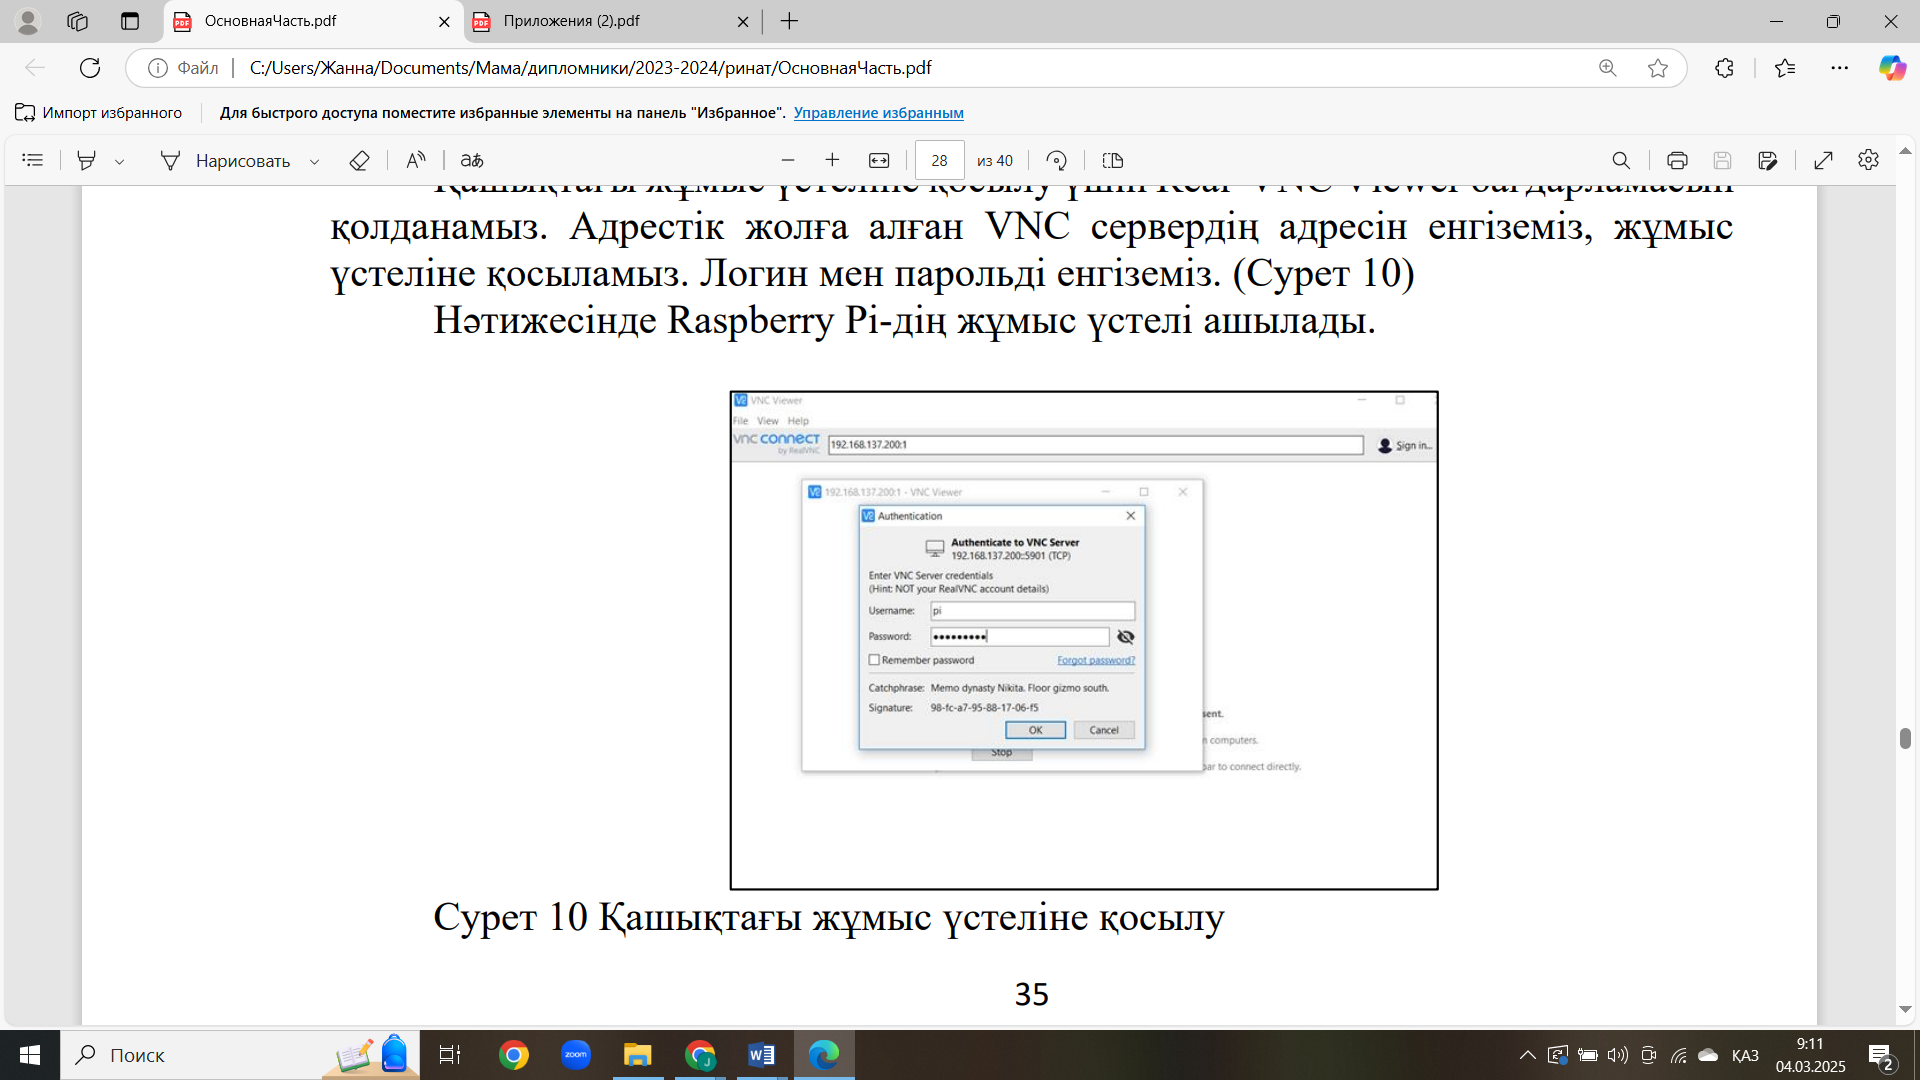
\includegraphics[width=0.8\textwidth]{media/ict2/image163}
	\caption*{4 - сурет. Қашықтағы жұмыс үстеліне қосылу}
\end{figure}

Face-recognition кітапханасы жұмыс істеу үшін dlib кітапханасын талап
етеді. Бірақ та dlib кітапханасының компиляциясы жедел жадының үлкен
көлемін алады, сондықтан оны орнатқан кезде жедел жадысына байланысты
қате шығады да, операциялық жүйе процесті бітіреді. Dlib кітапханасын
орнату алдында мүмкіндігінше жедел жадыны босатып алу керек. Ол үшін
жүктеу файлын үлкейтуге болады. Жүктеу файлы -- жүйенің жадысында
қосалқы виртуалды жад ретінде қолданылатын жады картасындағы бос орын.
Жүктеу файлы операциялық жүйеге нақты жадыдан көбірек жады бар екендей
көрсетуге мүмкіндік береді. Raspberry Pi операциялық жүйесінде жүктеу
файлы dphys-swapfile файлында әдепкі бойынша 100 МБ жадысымен беріледі.
Оны өзгерту үшін \$ sudo nano /etc/dphys-swapfile командасы арқылы осы
файлдың ішін ашамыз. CONF-SWAPSIZE=100 жолды 1024 мәнге өзгертеміз.
Жүктеу файлын өзгерткеннен кейін жүктеу сервисін \$sudo
/etc/init.d/dphys-swapfile stop \$sudo /etc/init.d/dphys-swapfile start
командалары арқылы қайтадан қосамыз. Содан кейін dlib орнату үшін cmake
программасы жазылады (\$ sudo apt-get install build-essential cmake).
Жүктеу файлы төмендегі 5 суретте көрсетілген.

\begin{figure}[H]
	\centering
	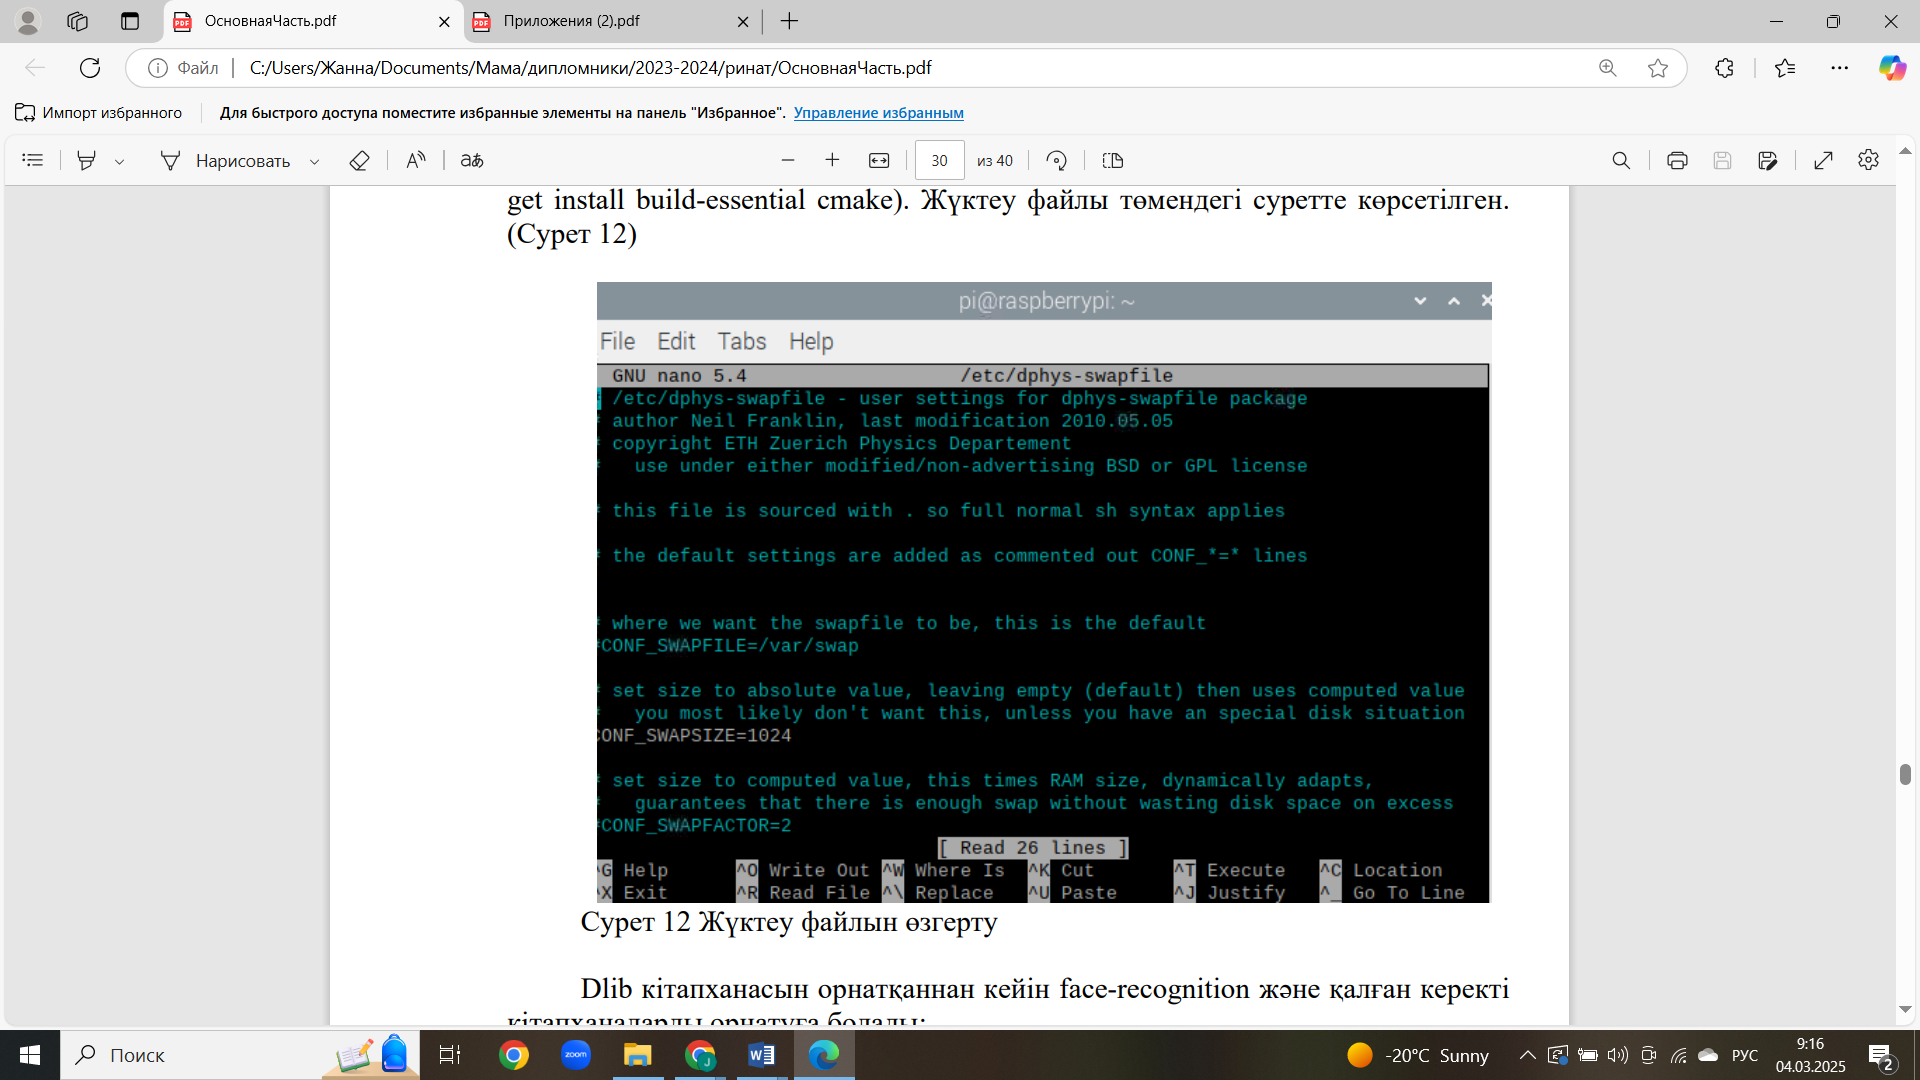
\includegraphics[width=0.8\textwidth]{media/ict2/image164}
	\caption*{5 - сурет. Жүктеу файлын өзгерту}
\end{figure}

\begin{multicols}{2}
Dlib кітапханасын орнатқаннан кейін face-recognition және қалған керекті
кітапханалар орнатылды: \$pip install face-recognition, deepface,
opencv-python, firebase-admin, datetime.

{\bfseries Қорытынды.} Зерттеу барысында Raspberry Pi платформасында
компьютерлік көру және жасанды интеллект әдістерін қолдану арқылы
қызметкерлердің эмоционалдық жағдайын тану жүйесі әзірленді және
енгізілді. Конволюционды нейрондық желілерге (CNN) негізделген
әзірленген алгоритм FER2013 сынақ деректер жинағында 92\%-ға жететін
эмоцияларды жіктеудің жоғары дәлдігін көрсетті, бұл дәстүрлі машиналық
оқыту әдістерінен жоғары.

Бет-әлпетті тану үшін негізгі құрал ретінде face-recognition кітапханасы
таңдалды, ал эмоцияны талдау үшін алдын ала дайындалған терең оқыту
үлгілерін пайдаланатын DeepFace таңдалды. Жүргізілген эксперименттер
нақты уақыт режимінде қызметкерлердің эмоционалдық күйлерін тиімді
анықтау және жіктеу мүмкіндігін растады.

Зерттеу нәтижелері қызметкерлердің психо-эмоционалдық жағдайын бақылау
үшін автоматты эмоцияларды талдау жүйелерін пайдалану уәдесін көрсетеді.
Бұл өнімділікті арттыру, күйіп қалуды болдырмау және жұмыс жағдайын
жақсарту сияқты салаларда қолданылуы мүмкін.

Әрі қарай зерттеулер күрделі модельдер мен қосымша параметрлер (стресс
деңгейі, шаршау) арқылы танылған эмоциялар жиынтығын кеңейтуге,
Raspberry Pi сияқты ресурсты көп қажет ететін платформаларда өңдеу
жылдамдығын арттыру үшін алгоритмдерді оңтайландыруға және
қызметкерлердің жағдайын жан-жақты бағалау үшін жүйені бақылаудың басқа
модульдерімен, соның ішінде сөйлеу және биометриялық деректерді
талдаумен интеграциялауға бағытталуы мүмкін.

Осылайша, әзірленген жүйе компьютерлік көру мен жасанды интеллект арқылы
қызметкерлердің мінез-құлқын интеллектуалды талдауға бағытталған маңызды
қадам болып табылады.
\end{multicols}

\begin{center}
{\bfseries Әдебиеттер}
\end{center}

\begin{references}
1. Jonathan K. Foster, Matthew Korban, Peter Youngs, Ginger S. Watson,
Scott T. Acton. Automatic classification of activities in classroom
videos// Computers and Education: Artificial Intelligence. -2024. -
Vol.6: 100207. \href{https://doi.org/10.1016/j.caeai.2024.100207}{DOI
10.1016/j.caeai.2024.100207}

2. Xiaohuan Song. Emotional recognition and feedback of students in
English e-learning based on computer vision and face recognition
algorithms// Entertainment Computing. -2025. - Vol.52, 100847.
\href{https://doi.org/10.1016/j.entcom.2024.100847}{DOI
10.1016/j.entcom.2024.100847}

3. Manuel A. Solis-Arrazola, Raul E. Sanchez-Yañez, Carlos H.
Garcia-Capulin, Horacio Rostro-Gonzalez. Enhancing image-based facial
expression recognition through muscle activation-based facial feature
extraction// Computer Vision and Image Understanding. -2024. - Vol.
240: 103927. \href{https://doi.org/10.1016/j.cviu.2024.103927}{DOI
10.1016/j.cviu.2024.103927}

4. Jianyang Zhang, Wei Wang, Xiangyu Li, Yanjiang Han. Recognizing facial
expressions based on pyramid multi-head grid and spatial attention
network// Computer Vision and Image Understanding. -2024. -
Vol.244:104010. \href{https://doi.org/10.1016/j.cviu.2024.104010}{DOI
10.1016/j.cviu.2024.104010}

5. Zhao X., Wang L., Zhang Y. et al. A review of convolutional neural
networks in computer vision// Artif Intell . - 2024. - Vol.57:99.
\href{https://doi.org/10.1007/s10462-024-10721-6}{DOI10.1007/s10462-024-10721-6}

6. Huang ZY., Chiang CC., Chen JH. et al. A study on computer vision for
facial emotion recognition// Sci Rep. -2023. -Vol.13: 8425.
\href{https://doi.org/10.1038/s41598-023-35446-4}{DOI
10.1038/s41598-023-35446-4}

7. Borriero A. et al. Explainable Emotion Decoding for~Human and~Computer
Vision// Communications in Computer and Information Science№ - 2024. -
Vol.2154. - P.178-201
\href{https://doi.org/10.1007/978-3-031-63797-1_10}{DOI
10.1007/978-3-031-63797-1\_10}

8. Esengalieva Zh., Oralbekova Zh., Turarova M. Medicina salasynda
komp' juterlіk kөru әdіsterіnің negіzіnde grafikalyқ
aқparatty өңdeu// ҚazTBU habarshysy. -2024. - T.3(24). - С.119-129.
\href{https://doi.org/10.58805/kazutb.v.3.24-423}{DOI
10.58805/kazutb.v.3.24-423}. {[}in Kazakh{]}

9. Batyr Z., Omarov B., Ziyatbekova G., Mailybayeva A. Traffic sign
recognition in challenging weather conditions using convolutional neural
networks//~Vestnik KazUTB. -2024. - Vol.2(23). - P.112-119.
\href{https://doi.org/10.58805/kazutb.v.2.23-471}{DOI
10.58805/kazutb.v.2.23-471}

10. Schroff, Florian and Kalenichenko, Dmitry and Philbin, James.
FaceNet: A unified embedding for face recognition and clusterin //2015
IEEE Conference on Computer Vision and Pattern Recognition (CVPR).~-
2015. ~- Р.~815--823.
\href{https://doi.org/10.1109/CVPR.2015.7298682}{DOI
10.1109/CVPR.2015.7298682}
\end{references}

\begin{authorinfo}
\emph{{\bfseries Авторлар туралы мәліметтер}}

Есенгалиева Ж.С. - PhD, доцент, Л.Н. Гумилев атындағы Еуразия ұлттық
университеті, Астана, Қазақстан, е-mail: jannayess@gmail.com;

Каиржан Р.С. - магистрант, Л.Н. Гумилев атындағы Еуразия ұлттық
университеті, Астана, Қазақстан, е-mail: kairzanrinat@gmail.com;

Глазырина Н.С. - PhD, доцент, Л.Н. Гумилев атындағы Еуразия ұлттық
университеті, Астана, Қазақстан, е-mail: glazirinan@yandex.ru;

\emph{{\bfseries Information about the authors}}

Yessengaliyeva Zh.S. - PhD, associate professor, Eurasian national
university, Astana, Kazakhstan е-mail: jannayess@gmail.com;

Kairzhan R.S. - master student, Eurasian national university, Astana,
Kazakhstan, е-mail: kairzanrinat@gmail.com;

Glazyrina N.S. - PhD, associate professor, Eurasian national university,
Astana, Kazakhstan, е-mail: glazirinan@yandex.ru.
\end{authorinfo}
